\documentclass{article}
\usepackage[utf8]{inputenc}
\usepackage{mathtools}
\usepackage{amssymb}
\usepackage{amsmath}
\usepackage{listings}
\usepackage{braket}
\usepackage[toc,page]{appendix}

%%%THEOREM (ETC) ENVIRONMENTS
\newtheorem{definition}{Definition}
\newtheorem{claim}{Claim}
\newtheorem{conjecture}{Conjecture}
\newtheorem{corollary}{Corollary}
\newtheorem{example}{Example}
\newtheorem{problem}{Problem}
\newtheorem{idea}{Idea} 

\usepackage{proof}
\newtheorem{theorem}{Theorem}

\newtheorem{lemma}[theorem]{Lemma}
\newtheorem{proposition}[theorem]{Proposition}

\newenvironment{proof}[1][Proof]{\begin{trivlist}
		\item[\hskip \labelsep {\bfseries #1}]}{\begin{flushright}$\blacksquare$\end{flushright} \end{trivlist}}
\newenvironment{remark}[1][Remark]{\begin{trivlist}
		\item[\hskip \labelsep {\bfseries #1}]}{\end{trivlist}}

\newcommand{\cat}{\mathcal{C}}
\newcommand{\Tau}{\mathrm{T}}
\newcommand{\ham}{\mathcal{H}}
\title{Hopf Algebras in Quantum Computation}
\author{Giovanni de Felice}
\date{April 2017}

%%%TIKZ:
\usepackage{tikz,pgfplots}
\usetikzlibrary{shapes.geometric}
\usetikzlibrary{trees, patterns}
\usetikzlibrary{positioning}
\usepackage{tikz,ifthen,calc}
\usepackage{tkz-euclide}
\usetikzlibrary{shapes,snakes}
\usetikzlibrary{calc,intersections, fit, knots, hobby, positioning, patterns}
\usepackage{braids}

%%%categorical diagrams:
\tikzset{
	buffer/.style={
		draw,
		shape border rotate=180,
		regular polygon,
		regular polygon sides=3,
		node distance=2cm,
		minimum height=4em
	}
}
\tikzstyle{arr}=[markings,mark=at position 0.5 with {\arrow{<}}]
%%%HOPF ALGEBRAS:
\newcommand{\mult}{
	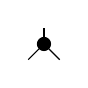
\begin{tikzpicture}[scale=0.2, black/.style={scale=0.5,draw,shape=circle,fill=black}]
	\node[black] (0) at (0, 0) {};
	\draw (1,-1) to (0);
	\draw (-1,-1) to (0);
	\draw (0) to (0,1);
	\end{tikzpicture}
}
\newcommand{\unit}{
	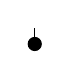
\begin{tikzpicture}[scale=0.2, black/.style={scale=0.5,draw,shape=circle,fill=black}]
	\node[black] (0) at (0, 0) {};
	\draw (0) to (0,1);
	\end{tikzpicture}
}
\newcommand{\comult}{
	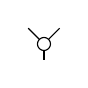
\begin{tikzpicture}[scale=0.2, black/.style={scale=0.5,draw,shape=circle,fill=white}]
	\node[black] (0) at (0, 0) {};
	\draw (1,1) to (0);
	\draw (-1,1) to (0);
	\draw (0) to (0,-1);
	\end{tikzpicture}
}

\newcommand{\counit}{
	\begin{tikzpicture}[scale=0.2, black/.style={scale=0.5,draw,shape=circle,fill=white}]
	\node[black] (0) at (0, 0) {};
	\draw (0) to (0,-1);
	\end{tikzpicture}
}

\newcommand{\antipode}{
	\begin{tikzpicture}[scale=0.2, black/.style={scale=0.5,draw,regular polygon,
		regular polygon sides=4,fill=white}]
	\node[scale=0.5, black] (0) at (0, 0) {$S$};
	\draw (0) to (0,-1);
	\draw (0) to (0,1);
	\end{tikzpicture}
}


\newcommand{\associativity}{
	\begin{equation}
	\begin{gathered}
	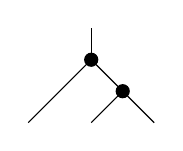
\begin{tikzpicture}[scale=0.8]
	\node[scale=0.5,draw,circle,fill=black] (0) at (0,0.5) {};
	\node[scale=0.5,draw,circle,fill=black] (1) at (0.5,0) {};
	\draw (0) to (1);
	\draw (-1,-0.5) to (0);
	\draw (0,-0.5) to (1);
	\draw (1,-0.5) to (1);
	\draw (0) to (0,1);
	\end{tikzpicture}
	\end{gathered}
	\, = \,
	\begin{gathered}
	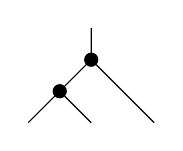
\begin{tikzpicture}[scale=0.8]
	\node[scale=0.5,draw,circle,fill=black] (0) at (0.5,0.5) {};
	\node[scale=0.5,draw,circle,fill=black] (1) at (0,0) {};
	\draw (0) to (1);
	\draw (-0.5,-0.5) to (1);
	\draw (0.5,-0.5) to (1);
	\draw (1.5,-0.5) to (0);
	\draw (0) to (0.5,1);
	\end{tikzpicture}
	\end{gathered}
	\end{equation}
}
\newcommand{\unitlaw}{
	\begin{equation}
	\begin{gathered}
	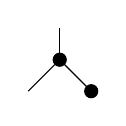
\begin{tikzpicture}[scale=0.8]
	\node[scale=0.5,draw,circle,fill=black] (0) at (0,0.5) {};
	\node[scale=0.5,draw,circle,fill=black] (1) at (0.5,0) {};
	\draw (0) to (1);
	\draw (-0.5,0) to (0);
	\draw (0) to (0,1);
	\end{tikzpicture}
	\end{gathered}
	\, = \,
	\begin{gathered}
	\begin{tikzpicture}[scale=0.8]
	\draw (0,0) to (0,1);
	\end{tikzpicture}
	\end{gathered}
	\, = \,
	\begin{gathered}
	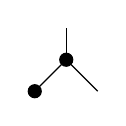
\begin{tikzpicture}[scale=0.8]
	\node[scale=0.5,draw,circle,fill=black] (0) at (0,0.5) {};
	\node[scale=0.5,draw,circle,fill=black] (1) at (-0.5,0) {};
	\draw (0) to (1);
	\draw (0.5,0) to (0);
	\draw (0) to (0,1);
	\end{tikzpicture}
	\end{gathered}
	\end{equation}
}
\newcommand{\coassociativity}{
	\begin{equation}
	\begin{gathered}
	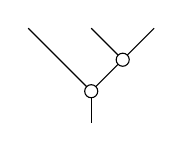
\begin{tikzpicture}[scale=0.8]
	\node[scale=0.5,draw,circle,fill=white] (0) at (0,-0.5) {};
	\node[scale=0.5,draw,circle,fill=white] (1) at (0.5,0) {};
	\draw (0) to (1);
	\draw (-1,0.5) to (0);
	\draw (0,0.5) to (1);
	\draw (1,0.5) to (1);
	\draw (0) to (0,-1);
	\end{tikzpicture}
	\end{gathered}
	\, = \,
	\begin{gathered}
	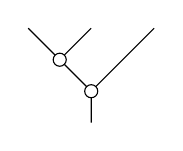
\begin{tikzpicture}[scale=0.8]
	\node[scale=0.5,draw,circle,fill=white] (0) at (0.5,-0.5) {};
	\node[scale=0.5,draw,circle,fill=white] (1) at (0,0) {};
	\draw (0) to (1);
	\draw (-0.5,0.5) to (1);
	\draw (0.5,0.5) to (1);
	\draw (1.5,0.5) to (0);
	\draw (0) to (0.5,-1);
	\end{tikzpicture}
	\end{gathered}
	\end{equation}
}
\newcommand{\counitlaw}{
	\begin{equation}
	\begin{gathered}
	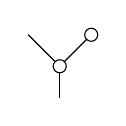
\begin{tikzpicture}[scale=0.8]
	\node[scale=0.5,draw,circle,fill=white] (0) at (0,-0.5) {};
	\node[scale=0.5,draw,circle,fill=white] (1) at (0.5,0) {};
	\draw (0) to (1);
	\draw (-0.5,0) to (0);
	\draw (0) to (0,-1);
	\end{tikzpicture}
	\end{gathered}
	\, = \,
	\begin{gathered}
	\begin{tikzpicture}[scale=0.8]
	\draw (0,0) to (0,1);
	\end{tikzpicture}
	\end{gathered}
	\, = \,
	\begin{gathered}
	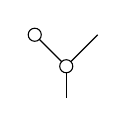
\begin{tikzpicture}[scale=0.8]
	\node[scale=0.5,draw,circle,fill=white] (0) at (0,-0.5) {};
	\node[scale=0.5,draw,circle,fill=white] (1) at (-0.5,0) {};
	\draw (0) to (1);
	\draw (0.5,0) to (0);
	\draw (0) to (0,-1);
	\end{tikzpicture}
	\end{gathered}
	\end{equation}
}

\newcommand{\bialgebralaw}{
	\begin{equation}
	\begin{gathered}
	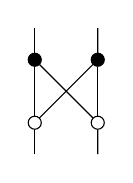
\begin{tikzpicture}[scale=0.8]
	\node[scale=0.5,draw,circle,fill=white] (0) at (0,0) {};
	\node[scale=0.5,draw,circle,fill=white] (1) at (1,0) {};
	\node[scale=0.5,draw,circle,fill=black] (2) at (0,1) {};
	\node[scale=0.5,draw,circle,fill=black] (3) at (1,1) {};
	\draw (0) to (2);
	\draw (0) to (3);
	\draw (1) to (2);
	\draw (1) to (3);
	\draw (0,-0.5) to (0);
	\draw (1,-0.5) to (1);
	\draw (0,1.5) to (2);
	\draw (1,1.5) to (3);
	\end{tikzpicture}
	\end{gathered}
	\, = \,
	\begin{gathered}
	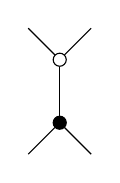
\begin{tikzpicture}[scale=0.8]
	\node[scale=0.5,draw,circle,fill=black] (0) at (0.5,0) {};
	\node[scale=0.5,draw,circle,fill=white] (1) at (0.5,1) {};
	\draw (0) to (1);
	\draw (0,-0.5) to (0);
	\draw (1,-0.5) to (0);
	\draw (0,1.5) to (1);
	\draw (1,1.5) to (1);
	\end{tikzpicture}
	\end{gathered}
	\end{equation}
}
\newcommand{\copylaw}{
	\begin{equation}
	\begin{gathered}
	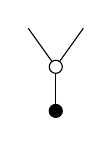
\begin{tikzpicture}[scale=0.7, squr/.style={scale=0.5,draw,regular polygon,
		regular polygon sides=4,fill=white}, black/.style={scale=0.5,draw,shape=circle,fill=black}, whit/.style={scale=0.5,draw,shape=circle,fill=white}]
	\node[black] (0) at (0, 0) {};
	\node[whit] (1) at  (0, 0.8) {};
	\draw (0) to (1);
	\draw (1) to (0.5,1.5);
	\draw (1) to (-0.5,1.5);
	\end{tikzpicture}
	\end{gathered}
	\, = \,
	\begin{gathered}
	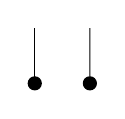
\begin{tikzpicture}[scale=0.7, black/.style={scale=0.5,draw,shape=circle,fill=black}]
	\node[black] (0) at (0,0) {};
	\node[black] (1) at (1,0) {};
	\draw (0) to (0,1);
	\draw (1) to (1,1);
	\end{tikzpicture}
	\end{gathered}
	\end{equation}
}
\newcommand{\cocopylaw}{
	\begin{equation}
	\begin{gathered}
	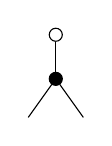
\begin{tikzpicture}[scale=0.7, squr/.style={scale=0.5,draw,regular polygon,
		regular polygon sides=4,fill=white}, black/.style={scale=0.5,draw,shape=circle,fill=black}, whit/.style={scale=0.5,draw,shape=circle,fill=white}]
	\node[whit] (0) at (0, 0) {};
	\node[black] (1) at  (0, -0.8) {};
	\draw (0) to (1);
	\draw (1) to (0.5,-1.5);
	\draw (1) to (-0.5,-1.5);
	\end{tikzpicture}
	\end{gathered}
	\, = \,
	\begin{gathered}
	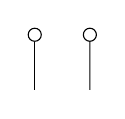
\begin{tikzpicture}[scale=0.7, black/.style={scale=0.5,draw,shape=circle,fill=white}]
	\node[black] (0) at (0,0) {};
	\node[black] (1) at (1,0) {};
	\draw (0) to (0,-1);
	\draw (1) to (1,-1);
	\end{tikzpicture}
	\end{gathered}
	\end{equation}
}
\newcommand{\hopflaw}{
	\begin{equation}
	\begin{gathered}
	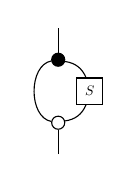
\begin{tikzpicture}[scale=0.8, squr/.style={scale=0.5,draw,regular polygon,
		regular polygon sides=4,fill=white}]
	\node[scale=0.5,draw,circle,fill=white] (0) at (0,0) {};
	\node[scale=0.5,draw,circle,fill=black] (1) at (0,1) {};
	\node[squr] (2) at (0.5,0.5) {$S$};
	\draw[bend left=80] (0) to (1);
	\draw[bend right] (0) to (2);
	\draw[bend right] (2) to (1);
	\draw (0,-0.5) to (0);
	\draw (0,1.5) to (1);
	\end{tikzpicture}
	\end{gathered}
	\, = \,
	\begin{gathered}
	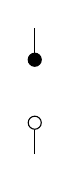
\begin{tikzpicture}[scale=0.8, squr/.style={draw,regular polygon,
		regular polygon sides=4,fill=white}]
	\node[scale=0.5,draw,circle,fill=white] (0) at (0,0) {};
	\node[scale=0.5,draw,circle,fill=black] (1) at (0,1) {};
	\draw (0,-0.5) to (0);
	\draw (0,1.5) to (1);
	\end{tikzpicture}
	\end{gathered}
	\, = \,
	\begin{gathered}
	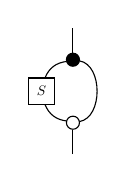
\begin{tikzpicture}[scale=0.8, squr/.style={scale=0.5,draw,regular polygon,
		regular polygon sides=4,fill=white}]
	\node[scale=0.5,draw,circle,fill=white] (0) at (0,0) {};
	\node[scale=0.5,draw,circle,fill=black] (1) at (0,1) {};
	\node[squr] (2) at (-0.5,0.5) {$S$};
	\draw[bend right=80] (0) to (1);
	\draw[bend left] (0) to (2);
	\draw[bend left] (2) to (1);
	\draw (0,-0.5) to (0);
	\draw (0,1.5) to (1);
	\end{tikzpicture}
	\end{gathered}
	\end{equation}
}
\newcommand{\modulelaw}{
	\begin{equation}
	\begin{gathered}
	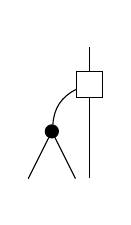
\begin{tikzpicture}[scale=0.6, squr/.style={draw,regular polygon,
		regular polygon sides=4,fill=white}, black/.style={scale=0.5,draw,shape=circle,fill=black}]
	\node (0) at (0, -2.2) {};
	\node[squr] (1) at (0, 0) {};
	\node (2) at (0, 1) {};
	\node[black] (3) at (-0.8, -1) {};
	\draw (0) to (1);
	\draw (1) to (2);
	\draw[bend left] (3) to (1);
	\draw (-1.3, -2) to (3);
	\draw (-0.3, -2) to (3);
	\end{tikzpicture}
	\end{gathered}
	\, = \,
	\begin{gathered}
	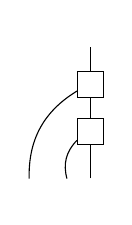
\begin{tikzpicture}[scale=0.6, squr/.style={draw,regular polygon,
		regular polygon sides=4,fill=white}, black/.style={draw,shape=circle,fill=black}]
	\node (0) at (0, -2.2) {};
	\node[squr] (1) at (0, 0) {};
	\node (2) at (0, 1) {};
	\node[squr] (3) at (0, -1) {};
	\draw (0) to (3);
	\draw (3) to (1);
	\draw (1) to (2);
	\draw (3) to (1);
	\draw[bend left] (-1.3, -2) to (1);
	\draw[bend left] (-0.5, -2) to (3);
	\end{tikzpicture}
	\end{gathered}
	\end{equation}
}
\newcommand{\comodulelaw}{
	\begin{equation}
	\begin{gathered}
	\begin{tikzpicture}[scale=0.6, squr/.style={draw,regular polygon,
		regular polygon sides=4,fill=white}, black/.style={scale=0.5,draw,shape=circle,fill=white}]
	\node (0) at (0, 2.2) {};
	\node[squr] (1) at (0, 0) {};
	\node (2) at (0, -2) {};
	\node[black] (3) at (-0.8, 1) {};
	\draw (0) to (1);
	\draw (1) to (2);
	\draw[bend right] (3) to (1);
	\draw (-1.3, 2) to (3);
	\draw (-0.3, 2) to (3);
	\end{tikzpicture}
	\end{gathered}
	\, = \,
	\begin{gathered}
	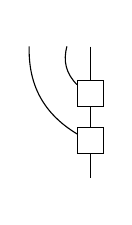
\begin{tikzpicture}[scale=0.6, squr/.style={draw,regular polygon,
		regular polygon sides=4,fill=white}, black/.style={draw,shape=circle,fill=black}]
	\node (0) at (0, 2.2) {};
	\node[squr] (1) at (0, 0) {};
	\node (2) at (0, -1) {};
	\node[squr] (3) at (0, 1) {};
	\draw (0) to (3);
	\draw (3) to (1);
	\draw (1) to (2);
	\draw (3) to (1);
	\draw[bend right] (-1.3, 2) to (1);
	\draw[bend right] (-0.5, 2) to (3);
	\end{tikzpicture}
	\end{gathered}
	\end{equation}
}
\newcommand{\intertwinerlaw}{
	\begin{equation}
	\begin{gathered}
	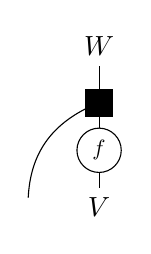
\begin{tikzpicture}[scale=0.6, squr/.style={draw,regular polygon,
		regular polygon sides=4,fill=black}]
	\node (0) at (0, -2.2) {$V$};
	\node[squr] (1) at (0, 0) {};
	\node (2) at (0, 1.2) {$W$};
	\node[scale=0.8,draw,circle] (3) at (0, -1) {$f$};
	\draw (0) to (3);
	\draw (3) to (1);
	\draw (1) to (2);
	\draw (3) to (1);
	\draw[bend left] (-1.5, -2) to (1);
	\end{tikzpicture}	
	\end{gathered}
	\, = \,
	\begin{gathered}
	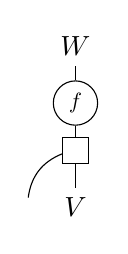
\begin{tikzpicture}[scale=0.6, squr/.style={draw,regular polygon,
		regular polygon sides=4,fill=white}]
	\node (0) at (0, -2.2) {$V$};
	\node[scale=0.8,draw,circle] (1) at (0, 0) {$f$};
	\node (2) at (0, 1.2) {$W$};
	\node[squr] (3) at (0, -1) {};
	\draw (0) to (3);
	\draw (3) to (1);
	\draw (1) to (2);
	\draw (3) to (1);
	\draw[bend left] (-1, -2) to (3);
	\end{tikzpicture}	
	\end{gathered}
	\end{equation}
}
\newcommand{\symAB}{
	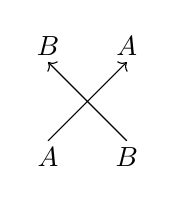
\begin{tikzpicture}[decoration={markings,mark=at position 0.5 with {\arrow{>}}}]
	\node (0) at (-0.5, -0.7) {$A$};
	\node (0) at (-0.5, 0.7) {$B$};
	\node (1) at (0.5, -0.7) {$B$};
	\node (1) at (0.5, 0.7) {$A$};
	\draw [->] (-0.5, -0.5) to (0.5, 0.5);
	\draw [->] (0.5, -0.5) to (-0.5, 0.5);
	\end{tikzpicture}
}

\newcommand{\symequation}{
	\begin{equation*}
	\begin{gathered}
	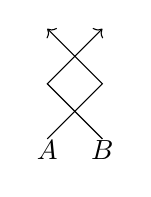
\begin{tikzpicture}[scale=0.7]
	\node (0) at (-1, -1.2) {$A$};
	\node (0) at (0, -1.2) {$B$};
	\draw [->] (-1, -1)--(0,0)--(-1,1);
	\draw [->] (0, -1)--(-1,0)--(0,1);
	\end{tikzpicture}
	\end{gathered}
	\, = \,
	\begin{gathered}
	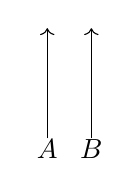
\begin{tikzpicture}[scale=0.7]
	\node (0) at (-0.8, -1.2) {$A$};
	\node (0) at (0, -1.2) {$B$};
	\draw [->] (-0.8, -1)--(-0.8,1);
	\draw [->] (0, -1)--(0,1);
	\end{tikzpicture}
	\end{gathered}
	\end{equation*}
}

\newcommand{\cupA}{	
	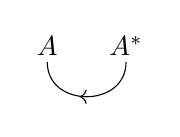
\begin{tikzpicture}[decoration={markings,mark=at position 0.5 with {\arrow{<}}}]
	\node (0) at (0, 0.2) {$A$};
	\node (1) at (1, 0.2) {$A^*$};
	\draw [bend right=90, looseness=1.5, postaction=decorate] (0,0) to (1,0);
	\end{tikzpicture}}

\newcommand{\capA}{	
	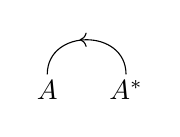
\begin{tikzpicture}[decoration={markings,mark=at position 0.5 with {\arrow{<}}}]
	\node (0) at (0, -0.2) {$A$};
	\node (1) at (1, -0.2) {$A^*$};
	\draw [bend left=90, looseness=1.5, postaction=decorate] (0,0) to (1,0);
	\end{tikzpicture}}

\newcommand{\snake}{
	\begin{equation*}
	\begin{gathered}
	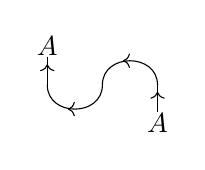
\begin{tikzpicture}[scale=0.7,decoration={markings,mark=at position 0.5 with {\arrow{<}}}]
	\node (0) at (0, 0.7) {$A$};
	\node (4) at (2, -0.7){$A$};
	\draw [bend right=90, looseness=1.5, postaction=decorate] (0, 0) to (1, 0);
	\draw [bend left=90, looseness=1.5, postaction=decorate] (1, 0) to (2, 0);
	\draw [postaction=decorate] (2, 0) to (2, -0.5);
	\draw [postaction=decorate] (0, 0.5) to (0, 0);
	\end{tikzpicture}
	\end{gathered}
	\, = \,
	\begin{gathered}
	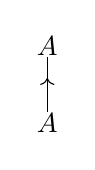
\begin{tikzpicture}[scale=0.7,decoration={markings,mark=at position 0.5 with {\arrow{<}}}]
	\node (0) at (0, 0.7) {$A$};
	\node (4) at (0, -0.7){$A$};
	\draw [postaction=decorate] (0, 0.5) to (0, -0.5);
	\end{tikzpicture}
	\end{gathered}
	\end{equation*}}

\newcommand{\snakestar}{
	\begin{equation*}
	\begin{gathered}
	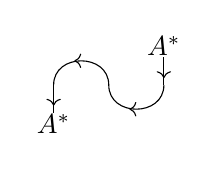
\begin{tikzpicture}[scale=0.7,decoration={markings,mark=at position 0.5 with {\arrow{<}}}]
	\node (0) at (0, -0.7) {$A^*$};
	\node (4) at (2, 0.7){$A^*$};
	\draw [bend left=90, looseness=1.5, postaction=decorate] (0, 0) to (1, 0);
	\draw [bend right=90, looseness=1.5, postaction=decorate] (1, 0) to (2, 0);
	\draw [postaction=decorate] (2, 0) to (2, 0.5);
	\draw [postaction=decorate] (0, -0.5) to (0, 0);
	\end{tikzpicture}
	\end{gathered}
	\, = \,
	\begin{gathered}
	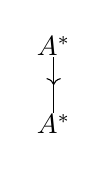
\begin{tikzpicture}[scale=0.7,decoration={markings,mark=at position 0.5 with {\arrow{>}}}]
	\node (0) at (0, 0.7) {$A^*$};
	\node (4) at (0, -0.7){$A^*$};
	\draw [postaction=decorate] (0, 0.5) to (0, -0.5);
	\end{tikzpicture}
	\end{gathered}
	\end{equation*}
}

\newcommand{\fusionijk}{
	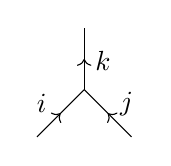
\begin{tikzpicture}[scale=0.6,decoration={markings,mark=at position 0.5 with {\arrow{>}}}]
	\node (0) at (-0.9, -0.3) {$i$};
	\node (1) at (0.9, -0.3) {$j$};
	\node (2) at (0.4, 0.6) {$k$};
	\draw [postaction=decorate] (-1, -1) to(0,0);
	\draw [postaction=decorate] (1,-1) to (0,0);
	\draw [postaction=decorate] (0,0) to (0,1.3);
	\end{tikzpicture}}
%%%%%%%%%%%%%%%%%%%%%%%%%%%%%%%%%%%%%%%%%%%%%%%%%%%%%%%%%%%%%%%%%%%%%%%%%%%%%%%%%%%%%%%%%%%%%%%%%%%%%%%%%%%%%%%%%%%%%%%%%%%%%%%%%%%%%%%%%%%%%%%%%%%%%%%%%%%%%%%%%%%%%%%%%%%%%%%%%%%%


\begin{document}


Classiclaly, there are three phases of matter: solid, liquid and gas. As temperature decreases we move from gas phase to liquid and solid phases. Close to zero temperature, phases of matter are quantized and we obtain exotic behaviours of matter. These are the contexts in which anyonic behaviour arises.\\
In order to talk about quantum phases of matter we need to consider many-body quantum systems. We will use the definitions of Zhenghan \cite{Rowell17}.

\begin{definition}[Many Body Quantum Systems]
	A Many-body Quantum system (MQS), is a triple $(\mathcal{L}, b, \mathcal{H})$, where $\mathcal{L}$ is a Hilbert space with a distinguished ONB $b$ and a hermitian operator $\mathcal{H}: \mathcal{L} \rightarrow \mathcal{L}$, called Hamiltonian.
\end{definition}
The eigenvalues of the Hamiltonian correspond to the energy levels of the system. The elements of the basis $b$ are the initial classical states of the system. Many-body quantum systems will usually be obtained from spatial configurations of particles, which we will describe by graphs.
\begin{definition}
	An MQS on a graph $\Tau = (V,E)$ with $\mathbb{C}^d$ degrees of freedom (qudit space) is an MQS $(\mathcal{L},b, \mathcal{H})$ where
	$$ \mathcal{L} = \otimes_{e\in E} \mathbb{C}^d$$
	$b$ is obtained from the standard basis of $\mathbb{C}^d$ and $\mathcal{H}$ is a local Hamiltonian.
\end{definition}
Where by local we mean the following.
\begin{definition}
	For an MQS on a graph, a Hamiltonian is $k$-local if it is of the form $\sum \mathcal{H}_i$ where each $H_I$ is of the form $id \otimes A \otimes id$ where $A$ acts on a disk of radius $k$ at a vertex in the edge length metric.
\end{definition}
Many interesting spatial configurations of matter are obtained from triangulations of manifolds by taking their 1-skeleton graph.\\
Let us consider unitary operators on $\mathcal{L}$ which commute with the Hamiltonian $\mathcal{H}$. That is they are unitary operators $U$ such that:
$$ U \ham U^\dagger = \ham$$
These are operators which leave the energy of the system unchanged. These transformations form a group $G$ under composition and a particle subject to the Hamiltonian $\mathcal{H}$ will be described by irreducible representations of $G$. $G$ is the group of symmetries of the system under $\mathcal{H}$.
\begin{proposition}
	Let $\mathcal{H}:V\rightarrow V$ be the Hamiltonian for some physical system described by a hilbert space $V$. Then the unitary operators which commute $\mathcal{H}$ form a group $G$.
\end{proposition}
\begin{proof}
	Suppose $R_1\ham=\ham R_1$ and $R_2\ham=\ham R_2$, then $R_1R_2\ham=R_1\ham R_2 = \ham R_1R_2$. Also $R^{-1}\ham = R^{-1}\ham RR^{-1} = R^{-1}R\ham R^{-1} =\ham R^{-1}$. The unit is the identity operator $id_{V^*\otimes V}$.
\end{proof}

\begin{proposition}
	If $G$ is the group of symmetries of a Hamiltonian $\mathcal{H}$ then each energy eigenspace carries an irreducible representation of $G$.
\end{proposition}
\begin{proof}
	Note that under the obvious $G$-action, $V$ is a representation of $G$. 
	The eigenvalues of the Hamiltonian, correspond to energy levels of the physical system which we previously called 'particle types'. Fix any eigenvalue $E$ of $\ham$, the allowed states of a particle with energy $E$ live in the corresponding eigenspace $V_E$. Indeed these are invariant under the action of $\ham$:
	$$ \ham \ket{\psi}= E\ket{\psi}$$
	Note that if $R\in G$ then
	$$ \ham R \ket{\psi}=R\ham \ket{\psi}=ER\ket{\psi}$$
	So $R\ket{\psi}$ is an eigenvector with eigenvalue $E$. Therefore $G$ acts on $V_E$ for any energy level.
	We prove $V_E$ is irreducible by showing that $End(V_E) \simeq \mathbb{C}$. Indeed suppose $f:V_E \rightarrow V_E$ is an intertwiner, then $fR=Rf \, \forall R \in G$
	TO PROVE
\end{proof}
Starting with a hamiltonian $\ham$ we have shown that energy levels (or particle types) correspond to the irreducible representations of the group $G$ of symmetries of $\ham$. The particle theory correponding to the hamiltonian $\ham$ has irreducible representations of $G$ as objects and intertwiners, preserving the energy of the system, as processes. This is the definition of the category $Rep(G)$. Note there are no restrictions yet on the group of symmetries.
\begin{definition}[Noether's theorem]
\end{definition}
In view of this fundamental result it is equivalent to consider symmetries...
\begin{example}
	Suppose $\ham = \sigma_Z$ be the Hamiltonian of a qubit living in $\mathbb{C}^2$. It has eigenvalues $\pm1$ and corresponding eigenvectors $\ket{0}$ and $\ket{1}$.. The group algebra of symmetries of $\ham$ is generated by $id$ and $\ham$ and it is isomorphic to $\mathbb{C}\mathbb{Z}_2$. $\mathbb{Z}_2$ has two irreducible representations (the trivial and the sign) representations which correspond to the one-dimensional eigenspaces of $\ham$. Note that 
\end{example}

%%%%%%%%%%%%%%%%%%%%%%%%%%%%%%%%%%%%%%%%%%%%%%%%%%%%%%%%%%%%%%%%%%%%%%%%%%%%%%%%%%%%%%%%%%%%%%%%%%%%%%%%%%%%%%%%%%%%%%%%%%%%%%%%%%%%%%%%%%%%%%%%
%%%%%%%%%%%%%%%%%%%%%%%%%%%%%%%%%%%%%%%%%%%%%%%%%%%%%%%%%%%%%%%%%%%%%%%%%%%%%%%%%%%%%%%%%%%%%%%%%%%%%%%%%%%%%%%%%%%%%%%%%%%%%%%%%%%%%%%%%%%%%%%%

Let us consider a two dimensional lattice of particles (situated on the edges of the lattice) under the influence of a magnetic field and an electric field. Anyonic behaviour is exhibited by excitations of the particles on the lattice. In our process theory the allowed processes are charge-flux composites, the states are lattice configurations (determined by the states of the particles, which are generally given by an element $g \in G$)  . By mearuring the flux in certain regions of the lattice and acting on the charge of the corresponding flux sector we can create and control the behaviour of excitations on the material.
\begin{example}
	Let us consider the case where $G \simeq \mathbb{Z}_2$. We obtain a lattice of spins. Those particles we wont use as our qubits, indeed we will impose that their state is in a basis state $\{\ket{0},\ket{1}\}$. One way to picture the states of the system is to draw the lattice and colour the edges red when the corresponding particle is in state $\ket{0}$. Note that the lattice can be embedded in any manifold (e.g. subsection quantum memory is a lattice on a torus, if we used a more layered lattice we could implement error correction). What we obtain is a picture of paths on the lattice which we call excitations.
\end{example}
The magnetic flux of a particle is given by an element $h \in G$, this indexes the superselection sectors so that the charge lives in a unitary irreducible representation of the centralizer $N(h)$ of the flux $h$ carried by the particle. We have two possible operations on our states: flux measurement and symmetry transformations on the charge. Flux measurements correspond to a projection $P_h \in \mathbb{C}G^*$ onto flux sector $h$. The residual global symmetry transformations are then implemented via some $g \in N(h)$. \\
Naturally the projectors form a Von Neumann family and satisfy 
$$P_hP_{h'}= \delta_{h,h'} P_h.$$ 
A general element $g \in G$ is a global symmetry transformation and affects the fluxes via conjugation:
\begin{equation}
gP_h = P_{ghg^{-1}}g
\end{equation}
The quantum double construction allows to capture both global symmetry transformations and projective measurements in one algebraic structure.
\begin{definition}
	For any finite group $G$, its quantum double $D(G)$ is the algebra generated by $\{P_hg\}_{h,g\in G}$ with multiplication induced by (1). $D(G) \simeq \mathbb{C}G^* \otimes \mathbb{C}G$ and inherits their hopf algebra structure (comultiplication and antipode are given by tensoring). 
\end{definition}
$D(G)$ has a natural quasi-triangular structure witnessed by the universal R-matrix $R=\sum_{g,h \in G}P_he \otimes P_hg$, making $RepDG$ braided. Particle states then live in irreducible representations of $D(G)$. Let $\{C_i\}_{i=1}^n$ be the distinct conjugacy classes in $G$. To each of those conjugacy classes corresponds a centralizer subgroup $N_i$ (two choices of representatives for $C_i$ yield isomorphic centralizer subgroups). Then for any irreducible representation $(\alpha,V^i_\alpha)$ of $N_i$ with basis elements $v^\alpha_j$, let $V_{i,\alpha} = \mathbb{C}C_i \otimes V^i_\alpha$, this has basis $\{ \ket{k,v^\alpha_j} \}_{j=1,...,dim\alpha}^{k\in C_i}$ and forms an irreducible representation of $D(G)$ under the action 
\begin{equation}
P_hg\ket{k,v^\alpha_j} = \delta_{h,gkg^{-1}} \ket{h,\alpha(h^{-1}gk)v^\alpha_j}
\end{equation}
and the $\{V_{i,\alpha}\}$ is the complete set of irreducible representations.

%%%%%%%%%%%%%%%%%%%%%%%%%%%%%%%%%%%%%%%%%%%%%%%%%%%%%%%%%%%%%%%%%%%%%%%%%%%%%%%%%%%%%%%%%%%%%%%%%%%%%%%%%%%%%%%%%%%%%%%%%%%%%%%%%%%%%%%%%%%%%%%%
%%%%%%%%%%%%%%%%%%%%%%%%%%%%%%%%%%%%%%%%%%%%%%%%%%%%%%%%%%%%%%%%%%%%%%%%%%%%%%%%%%%%%%%%%%%%%%%%%%%%%%%%%%%%%%%%%%%%%%%%%%%%%%%%%%%%%%%%%%%%%%%%

\begin{remark}
	Can we generalise the lattice construction?
	The following argument seems to work for abelian groups.
	Being a spherical fusion category, $RepG$ is well suited to be a process theory of particles. As we pointed out earlier what is missing is the braided structure, but let us ignore this for the moment. We have simple objects corresponding to particle types and fusion rules determined by the group structure.\\
	Now suppose we have particles whose fusion is described by a $RepG$ and let us consider a lattice with those particles located at the edges. This lattice could be embedded in any space but let us assume it is a lattice on a torus. The states of our system are then configurations of particle types on the edges. So edges are coloured by simple representations from $RepG$. Now we can act on the lattice with vertex and plaquette operators which basically implement measurements at vertices and flips (fusion with other simple reps) of the particles on a plaquette. By now we have produced a theory where states are lattice configurations and processes are generated by vertex $V_\alpha$ and plaquette $P_\beta$ operators. We want to extract the topological degrees of freedom of this theory. First we note that using vertex operators we can make sure that the product of all particles incident at all vertices is 1, i.e $V_\alpha=1$ $\forall \alpha$. We restrict our states to satisfy this local property and we drop vertex operators (in the sense that they are not allowed processes anymore), indeed we fixed their value at all points of the lattice. By also setting $P_\beta =1$ at all plaquettes we quotient further the theory. So we obtain a theory where all vertex and plaquette measurements have value $1$. We finally declare two configurations to be equal if there is a sequence of plaquette operations taking us from one to the other. Noting that plaquette operators are local isometries we see this corresponds to quotienting out the category by an equivalence relation. This doesn't exaust the degrees of freedom of the theory because of the topology of the torus. Those topological degrees of freedom will be the simple objects our newly created category, their fusion rules are completely determined by the structure of $Rep(G)$. Indeed the category we obtained is $Z(Rep(G)) \simeq Rep(DG)$.	
\end{remark}

\begin{example}
	In the case $G=\mathbb{Z}_2$, recall $Rep\mathbb{Z}_2$ has two simple object of dimension one $\tau_+$ and $\tau_-$ with fusions given by group structure. Let us draw the states of our system as colourings of the edges of the lattice. The condition on the vertex operators results in no endlines and no triple intersections on the lattice. The condition on plaquette operators only allows loop configurations. Quotienting out by plaquette operators relation we obtain 4 distinct classes, namely the vacuum $1$, the first cycle of the torus $X$, the second cycle $Z$, and both cycles $X \otimes Z \simeq Y$ and we have the fusion rules. The theory we have obtained is $RepD\mathbb{Z}_2$ which has in fact 4 simple objects with same fusions. We are therefore treating the topological defects of a theory in $Rep\mathbb{Z}_2$ as particles particles in their own right, with their own theory. All those representations are one-dimensional and in fact we just formulated a theory of abelian anyons.
\end{example}

\begin{example}[Anyon Vacuum on a Torus and Quantum Memory]
	If we consider the torus as our configuration space. Let $C_1$, $C_2$ be the two cycles. Consider the process $T_i$ for $i=1,2$ which creates a particle-antiparticle pair, moves them in opposite directions around cycle $C_i$ so that they meet on the other side of the torus and annihilate. Then we can show $T_i$ do not commute with each other if the particles are abelian anyons with $\theta \neq 0, \pi$. We know $\theta$ must be a fraction $p/q$ with $p$ and $q$ coprime. Then we can show that the system has degenerate ground states. We have $q$ different ground state, so the vacuum state lives in a $q$ dimensional space. If we initialise it in some superposition it will remain in that state unless a $T_1$ or $T_2$ operation is implemented. Because of their topological nature it is very unlikely that such processes occur spontaneously, and therefore the quantum information stored in the superposition is protected.
\end{example}

\subsection{An adjunction between fPQC and TQC}
This section is dedicated to the relationship between a category $\mathcal{C}$ and its braided centre $Z(\mathcal{C})$. In the first part we will talk about non-commutative logic and modalities. In the second part we will see \\

Free forgetful adjunction:
$$\Box: \mathcal{C} \rightleftarrows Z(\mathcal{C}):U$$ \\


$$\Box: RepG \rightarrow RepDG\simeq Z(RepG)$$
\begin{theorem}
	Let $\{X_i\}_{i\in I}$ be the set of representatives of the isomorphism classes of simple objects in $RepG$. Let $\mathbb{C}G$ be the regular representation, then $$\mathbb{C}G \simeq \oplus_{i\in I}X_i\otimes X_i^*$$
\end{theorem}
\begin{theorem}
	$\Box V = \oplus_{i\in I}X_i^*\otimes V \otimes X_i$ with action of $DG$ given by ....
\end{theorem}
Let $G$ be a group, $DG$ its quantum double, $(\pi,V)$ a representation of $G$. \\
The induced representation $\Box V$ is the coequalizer of: \\
$$DG \otimes \mathbb{C}G \otimes V \rightrightarrows DG\otimes V$$ 
Where the top arrow is given by the right action of $G$ on $DG \simeq \mathbb{C}G^* \otimes \mathbb{C}G$ 
$$ (P_hg, k) \mapsto P_h (gk^{-1})$$
(this satisfies the axioms of an action but do we have to make the action conjugate the flux projection component?) and the bottom arrow is given by the $\pi$ action on $V$. \\
To compute the coequalizer we consider the orbits of the action of $G$ on $DG$, these form a partition of $DG$:
$$ \{[P_ke] : k \in G\} $$
So, as a vector space $\Box V \simeq \mathbb{C}G \otimes V$ and the action of $DG$ on $\Box V$ is given by:
\begin{equation}
P_hg [P_ke]v = \delta_{h,gkg{-1}} [P_he] \pi(g)v
\end{equation} 
So that element $P_hg$ implements residual symmetry $g$ and projects onto flux sector $gkg^{-1}$. \\
Note that if $C_i$ are the conjugacy classes of $G$ then $\mathbb{C}G \simeq \oplus_i \mathbb{C}C_i$ and we could try to decompose:
\begin{equation}
\Box V \simeq \oplus_i \mathbb{C}C_i \otimes V
\end{equation}
The action (3) factors through the conjugacy classes, (4) gives us a decomposition of $ \Box V$ into irreducibles if $V$ is simple in $RepG$? (this hold for abelian groups, should be generalised given decomposition of $V$ into $Z_i$ modules). \\
$\Box$ is clearly not monoidal if we take $\otimes$ as tensor, is it monoidal under $\oplus$? i.e is it additive? (Note that the induced representation functor $Ind_H^G$ for $H$ subgroup of $G$ is additive). If it is additive then it is left and right exact and could use this to find the decomposition of $ \Box V$ \\
Is the $\Box$ functor representable? In the sense $\Box \simeq Hom(\mathbb{C}G,\_)$?


\begin{example}
	If $G=\mathbb{Z}_2= \{e,a\}$, irreducible representations are the trivial $\tau_+$ and the one dimensional sign representation $\tau_-$. $DG \simeq \mathbb{C}\mathbb{Z}_2^* \otimes \mathbb{C}\mathbb{Z}_2$ and the orbits of the right action of $\mathbb{Z}_2$ on $D\mathbb{Z}_2$ are given by
	$$ \{ [P_ee], [P_ae] \}$$
	Recall that $D\mathbb{Z}_2$ has 4 irreducible one dimensional representations which we denoted $1$,$X$,$Z$,$Y$. With fusion rules generated by $A \otimes A \simeq 1$ and $X \otimes Y \simeq Z$. \\
	Now let us calculate $\Box \tau_-$, it has basis $\{[P_ee] =:w_e, [P_ae] =:w_a \}$ and 
	\begin{equation*}
	P_ee(xw_e + yw_a)= xw_e \\
	P_ae(xw_e + yw_a)= yw_a \\
	P_ea(xw_e + yw_a)= -xw_e \\ 
	P_aa(xw_e + yw_a)= -yw_a
	\end{equation*}
	And we see from the table (see Lahtinen "The Toric Code and the Quantum Double" for table of reps) that $\Box \tau_- \simeq X \oplus Y$. Similarly $\Box \tau_+ \simeq 1 \oplus Z$. \\
	Consider the regular representation $V := \mathbb{C}\mathbb{Z}_2 \simeq \tau_+ \oplus \tau_-$, then $\Box V \simeq 1 \oplus X \oplus Z \oplus Y \simeq (1 \oplus X) \otimes (1 \oplus Z) $.\\
	What happens if we braid the two components of $\Box V$? In $RepD\mathbb{Z}_2$ the braid is implemented by acting on the components with $R=\sum_{g,h\in\mathbb{Z}_2} P_ge \otimes P_gh \, \in D\mathbb{Z}_2\otimes D\mathbb{Z}_2$ and swapping coordinates. I claim this implements a CNOT gate followed by a swap.
\end{example}

\begin{example}
	If $G=S_3=\braket{\sigma,\rho}$ where $\sigma$ is a reflection and $\rho$ a rotation. $S_3$ has three irreducible representations: the trivial $\tau_+$, the sign representation $\tau_-$ and the two dimensional $\tau_2$.
\end{example}

\end{document}
%%%%%%%%%%%%%%%%%%%%%%%%%%%%%%%%%%%%%%%%%%%%%%%%%%%%%%%%%%%%%%%%%%%%%%%%%%%%%%%%%%%%%%%%%%%%%%%%%%%%%%%%%%%%%%%%%%%%%%%%%%%%%%%%%%%%%%%%%%%%%%%%
%%%%%%%%%%%%%%%%%%%%%%%%%%%%%%%%%%%%%%%%%%%%%%%%%%%%%%%%%%%%%%%%%%%%%%%%%%%%%%%%%%%%%%%%%%%%%%%%%%%%%%%%%%%%%%%%%%%%%%%%%%%%%%%%%%%%%%%%%%%%%%%%
